% Fairness Is Advantage-Neutral -- manuscript source (reconstructed from the v1.0.0 PDF,
% with the bibliography moved to refs.bib and citations completed throughout).
% Build:  tectonic main.tex      (or: pdflatex main && bibtex main && pdflatex main && pdflatex main)
\documentclass[11pt,a4paper]{article}

\usepackage{amsmath,amsthm,mathtools}
\usepackage{newpxtext,newpxmath}
\usepackage[a4paper,margin=27mm]{geometry}
\usepackage{graphicx,booktabs,array,enumitem}
\usepackage{algorithm}
\usepackage[noend]{algpseudocode}
\usepackage{tikz}
\usepackage{quantikz}
\usepackage[numbers,sort&compress]{natbib}
\usepackage{xcolor}
\usepackage{microtype}
\usepackage{xurl}
\usepackage[colorlinks=true,linkcolor=black,citecolor=black,urlcolor=black]{hyperref}

% ---------------------------------------------------------------- theorem styles
\newtheorem{theorem}{Theorem}
\newtheorem{definition}[theorem]{Definition}

% ---------------------------------------------------------------- notation
\newcommand{\R}{\mathbb{R}}
\newcommand{\E}{\mathbb{E}}
\newcommand{\one}{\mathbf{1}}
\newcommand{\F}{F}
\newcommand{\PXP}{\mathrm{PXP}}
\newcommand{\KL}{\mathrm{KL}}
\newcommand{\TV}{\mathrm{TV}}
\newcommand{\FAIR}{\textsc{Fair}}
% \ket and \bra are provided by quantikz
\DeclareMathOperator*{\argmax}{arg\,max}
\DeclareMathOperator{\conv}{conv}
\DeclareMathOperator{\relint}{relint}
\DeclareMathOperator{\Var}{Var}
\DeclareMathOperator{\poly}{poly}

\title{\textbf{Fairness Is Advantage-Neutral:}\\[2pt]
\textbf{Guided Quantum Gibbs Dynamics for Fair Allocation}\\
\textbf{of Indivisible Resources}}
\author{Arnav Sharma, \ Arushi Uppal, \ Ritesh Roshan Sahoo, \ Krish Sabharwal\\[4pt]
\normalsize School of Artificial Intelligence, Amrita Vishwa Vidyapeetham\\
\normalsize Faridabad, Haryana, India}
\date{}

\setlength{\emergencystretch}{2.5em}

\begin{document}
\maketitle

\begin{abstract}
Fair allocation of scarce indivisible resources is a natural target for quantum optimisation,
but fairness criteria such as max-min welfare and the Gini coefficient cannot be written as
quadratic binary objectives without auxiliary variables. We show that this obstruction disappears
once allocations are randomised. By convex duality every concave fairness criterion reduces to a
weighted-welfare problem whose Hamiltonian has the degree of the valuations, at zero auxiliary cost,
and ex-ante fair allocation is polynomially equivalent to weighted-welfare allocation on any
computational model. Fairness is therefore advantage-neutral: a quantum speedup for fair allocation
exists exactly when one exists for the underlying combinatorial problem. Repeated fair allocation
becomes a multiplicative-weights game whose rounds are Gibbs sampling problems with slowly varying
targets. We prove a regret guarantee and a warm-start theorem under which each round costs a number
of chain steps set by the spectral gap alone. For fair scheduling under interference we construct a
quantum-enhanced Metropolis sampler whose proposals come from a palindromic Trotterisation of a cost
Hamiltonian plus the blockade-preserving PXP driver. We prove that the circuit never leaves the
feasible set, that the proposal is exactly symmetric at every Trotter depth, and that the chain
converges to the fair Gibbs lottery. We give the circuit at gate level with closed-form resource
counts and verify it against exact simulation to $10^{-15}$. On three graph families with up to
twenty links, quantum proposals enlarge the spectral gap over local moves by factors of 3.4 to over
1000, with geometric means of 20 to 49 per family. On Erd\H{o}s--R\'enyi graphs the fitted
gap-scaling exponent improves on the best classical baseline by a factor of $1.9\pm0.5$ to
$2.3\pm0.8$, but not on unit-disk or random 3-regular graphs. In repeated max-min allocation the
quantum-mixed chain reaches a fairness value of $1.327\pm0.007$ against $1.179\pm0.139$ classically,
with ex-ante optimum $1.460$. These results establish constant-factor and instance-dependent gains,
not a general quantum advantage.
\end{abstract}

\noindent\textbf{Keywords:} fair division; quantum optimisation; Markov chain Monte Carlo; convex
duality; independent sets; Rydberg arrays

% =====================================================================
\section{Introduction}

Consider a small example. Alice and Bob share three radio transmitters along a corridor
(Figure~\ref{fig:story}). Neighbouring transmitters interfere: $a$ and $b$ cannot transmit at the same
time, and neither can $b$ and $c$, but $a$ and $c$ are far enough apart. Alice owns $a$ and $c$, Bob owns
$b$, and every transmitter sends one packet when it fires. In every time slot a scheduler must decide
which transmitters fire.

Only two choices are worth making. Firing $a$ and $c$ gives Alice two packets and Bob none. Firing $b$
gives Bob one packet and Alice none. Every choice therefore leaves someone with nothing. A scheduler
that maximises the total always picks $\{a,c\}$, and Bob is never served.

The way out is to randomise. If the scheduler fires $\{a,c\}$ in one third of the slots and $\{b\}$ in
the other two thirds, Alice expects $2\cdot\frac13=\frac23$ of a packet per slot and Bob expects
$1\cdot\frac23=\frac23$. No rule does better for whoever is worse off, since raising either share lowers
the other. Lotteries of this kind are already used to ration scarce medical
treatments~\cite{white2022multicenter,pathak2024fair}.

The scheduler does not need to know the split $\frac13:\frac23$ in advance. It keeps a priority for
Alice and one for Bob, fires the schedule with the larger priority-weighted value, and afterwards
lowers the priority of whoever was just served. The priorities settle near $(\frac13,\frac23)$, which
are exactly the weights at which the two schedules tie, because $\frac13\cdot2=\frac23\cdot1$. Two things
are worth noticing. Fairness entered only through the priorities. And the only question the scheduler
ever answered was the ordinary one: which schedule is best at these priorities?

With thousands of transmitters, that question becomes the maximum-weight independent set problem,
which is NP-hard~\cite{garey1979computers}. So instead of finding the best schedule, the scheduler draws
a good one at random with a random walk that switches one transmitter on or off at a time. Here the walk
is slow. To get from $\{a,c\}$ to $\{b\}$ it must switch $a$ off, then $c$ off, then $b$ on, passing
through schedules that are worse for everyone.

Now replace the transmitters by atoms, one per transmitter, held in a Rydberg array. Two excited atoms
that are too close cannot coexist (the Rydberg blockade~\cite{jaksch2000fast,bernien2017probing}), so if
the atoms are placed like the transmitters, the physics itself forbids every schedule that interferes.
Let the atoms evolve for a short time and then measure them: the result is a proposed schedule, and it
can jump from $\{a,c\}$ to $\{b\}$ in one move. A classical coin then accepts or rejects the proposal so
that, in the long run, each schedule is used exactly as often as the fair lottery
requires~\cite{metropolis1953equation,layden2023quantum}.

What did the quantum device contribute? Not fairness: the priorities took care of that. It made the
random walk faster. This paper shows that this is true in general. Once lotteries are allowed,
fairness never makes allocation harder, and the only place a quantum device can help a fair
allocator is in finding or sampling good schedules.

\begin{figure}[t]
\centering
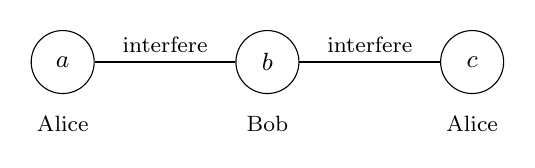
\begin{tikzpicture}[every node/.style={font=\small}]
\foreach \x/\n/\who in {0/a/Alice,2.6/b/Bob,5.2/c/Alice}{
  \node[draw,circle,thin,minimum size=8mm] (\n) at (\x,0) {$\n$};
  \node[below=1.5mm of \n,font=\footnotesize] {\who};}
\draw[thin] (a)--node[above,font=\footnotesize]{interfere}(b);
\draw[thin] (b)--node[above,font=\footnotesize]{interfere}(c);
\end{tikzpicture}
\caption{Three transmitters along a corridor. Neighbours interfere, so $a$ and $b$ cannot transmit
together, nor can $b$ and $c$; $a$ and $c$ can. Alice owns $a$ and $c$, Bob owns $b$.}
\label{fig:story}
\end{figure}

The example is small, but its structure is general: allocating food, vaccines, ventilators, spectrum or transmission slots under scarcity is an equity
problem as much as an efficiency problem~\cite{moulin2003fair,brandt2016handbook,pathak2024fair,bertsimas2011price}.
Welfare economics offers many ways of stating what a fair allocation is, from Rawlsian max-min and
leximin~\cite{rawls1971theory} through the Gini and Atkinson families~\cite{atkinson1970measurement,sen1973economic,weymark1981generalized}
to Nash welfare~\cite{nash1950bargaining,kaneko1979nash} and envy-based
criteria~\cite{foley1967resource,varian1974equity}. Quantum optimisation hardware accepts a much
narrower input: a quadratic objective over binary variables, or its Ising
equivalent~\cite{lucas2014ising,kadowaki1998quantum,farhi2014quantum}. Max-min welfare has
multilinear degree up to the number of agents, and absolute differences, and hence the Gini
coefficient, have degree at least three (Section~\ref{sec:prices}). Neither can be written as a
quadratic binary objective without auxiliary variables and penalties~\cite{boros2002pseudo}.
Published quantum treatments of equity therefore either substitute a quadratic surrogate for the
intended criterion~\cite{udekwe2025qrestore} or move the fairness objective out of the Hamiltonian
altogether~\cite{bach2026learning}.

As the example shows, when goods are indivisible the object of fair allocation is a lottery over
allocations rather than a single allocation~\cite{diamond1967cardinal,aziz2024best,harsanyi1955cardinal}, and randomised
rationing is already used for scarce medical resources~\cite{white2022multicenter,pathak2024fair}.
Over lotteries the attainable utility set is convex. Convex duality~\cite{rockafellar1970convex}
then separates the normative content of a fairness criterion from the combinatorial content of the
feasible set, and this separation settles both the representation question and the question of
where a quantum device can help.

\paragraph{Contributions.}
\begin{enumerate}[leftmargin=*]
\item A normative--combinatorial separation theorem (Theorem~\ref{thm:sep}). Every concave fairness
criterion, together with any requirement linear in the lottery, reduces to weighted-welfare best
responses at zero auxiliary cost.
\item Advantage neutrality (Theorem~\ref{thm:neutral}): ex-ante fair allocation and weighted-welfare
allocation are polynomially equivalent on every computational model.
\item A dynamic formulation of repeated fair allocation with a regret guarantee
(Theorem~\ref{thm:dyn}) and a warm-start theorem (Theorem~\ref{thm:warm}) that bounds the per-round
sampling cost by the spectral gap, with no dependence on the size of the state space.
\item A quantum proposal for fair scheduling under interference that preserves feasibility exactly
and is exactly symmetric at every Trotter depth, yielding a chain with the fair Gibbs lottery as its unique stationary
distribution (Theorem~\ref{thm:correct}). The circuit is given at gate level with closed-form
counts.
\item An open, verified implementation and an experimental study on three graph families with five
classical and quantum kernels, including exact warm-start tracking costs along
multiplicative-weights trajectories.
\end{enumerate}

The results are deliberately scoped. The theory shows that fairness cannot be the source of a
quantum advantage. The experiments show where constraint-native quantum proposals help a fair
sampler and where they do not. On present evidence, no general quantum advantage is claimed.

% =====================================================================
\section{Related work}\label{sec:related}

Four lines of work meet in this paper. Each has solved one part of the problem and left another
open, and the gap they leave together is the one we address.

\paragraph{What fairness means, and why lotteries.}
Inequality measurement starts from the transfer principle~\cite{dalton1920measurement} and the
equally-distributed-equivalent income of Atkinson~\cite{atkinson1970measurement}; Sen and Weymark
turned the Gini coefficient into a welfare function~\cite{sen1973economic,weymark1981generalized},
and the generalized Lorenz order is the consensus of all Schur-concave
criteria~\cite{shorrocks1983ranking,marshall2011inequalities}. Between the utilitarian
sum~\cite{harsanyi1955cardinal} and Rawlsian max-min~\cite{rawls1971theory} lie Nash
welfare~\cite{nash1950bargaining,kaneko1979nash}, $\alpha$-fairness~\cite{mo2000fair},
Kalai--Smorodinsky~\cite{kalai1975other} and ordered weighted averages~\cite{yager1988ordered};
which of these is admissible depends on the informational basis of the
comparison~\cite{hammond1976equity,daspremont1977equity}, and each has an efficiency
price~\cite{bertsimas2011price}. For indivisible goods, exact fairness generally fails: envy-freeness
up to one good exists~\cite{lipton2004approximately,budish2011combinatorial}, maximin shares need
not~\cite{kurokawa2018fair}, and envy-freeness up to any good fails for submodular
valuations~\cite{akrami2026counterexample}. The classical remedy, anticipated in the
Harsanyi--Diamond exchange~\cite{harsanyi1955cardinal,diamond1967cardinal}, is to randomise:
lotteries recover exact ex-ante fairness with approximate ex-post
guarantees~\cite{aziz2024best}, although ex-ante envy-freeness with Pareto optimality is
PPAD-hard~\cite{caragiannis2023complexity} and variance-based objectives are
NP-hard~\cite{babaioff2026best}. Weighted lotteries are now used to ration scarce
therapeutics~\cite{white2022multicenter,pathak2024fair}. Most relevant here, Kawase and
Sumita~\cite{kawase2020maxmin} showed that a max-min fair lottery can be computed by repeatedly
maximising a weighted utilitarian welfare. \emph{Left open:} a single statement covering every concave
criterion, and what it implies for the computational model on which the weighted problem is solved.

\paragraph{Fairness as prices on a feasible set.}
Convex duality~\cite{fenchel1949conjugate,rockafellar1970convex,sion1958general} turns a
concave objective over a polytope into a sequence of linear ones, and convex optimisation over a polytope
reduces in polynomial time to linear optimisation over it~\cite{grotschel1988geometric}.
Multiplicative weights~\cite{freund1997decision,freund1999adaptive,arora2012multiplicative}
realise the dual as a repeated game with regret
guarantees~\cite{cesabianchi2006prediction}. Wireless networking arrived at the same structure
independently: max-weight scheduling solves a weighted independent-set problem in every
slot~\cite{tassiulas1992stability}, $\alpha$-fair congestion control sets the
weights~\cite{mo2000fair}, adaptive CSMA replaces the maximisation by Gibbs sampling over
independent sets with dual weights~\cite{jiang2010distributed}, and the network adiabatic
theorem shows that the sampler tracks slowly varying weights~\cite{rajagopalan2009network}.
\emph{Left open:} all of these samplers use local (Glauber) moves, and local chains on independent
sets mix exponentially slowly at high weights, where sampling is provably
hard~\cite{mossel2009hardness,sly2010computational}. The kernel, not the fairness rule, is the
bottleneck.

\paragraph{Quantum optimisation, and why fairness has resisted it.}
Quantum annealers and variational circuits take a quadratic binary objective, or its Ising
form~\cite{lucas2014ising,kadowaki1998quantum}. The quantum approximate optimisation
algorithm~\cite{farhi2014quantum} alternates cost and mixing Hamiltonians; constraint-preserving
mixers remove equality penalties~\cite{hadfield2019quantum,wang2020xy}; low-depth circuits face
locality and symmetry obstructions~\cite{farhi2020quantum,bravyi2020obstacles}; and quadratic
speedups are unlikely to survive error-correction overheads~\cite{babbush2021focus}. Larger speedups
need structure: algebraic structure in decoded quantum
interferometry~\cite{jordan2025optimization,anschuetz2025decoded}, planted
structure~\cite{schmidhuber2025quartic}, or sign-problem-free adiabatic
paths~\cite{gilyen2021subexponential,hastings2021power}. Maximum independent set is native to Rydberg
arrays through the blockade
mechanism~\cite{jaksch2000fast,lukin2001dipole,pichler2018quantum,bernien2017probing,ebadi2022quantum},
but classical solvers remain competitive on unit-disk instances~\cite{andrist2023hardness}, general
graphs need embedding gadgets~\cite{nguyen2023quantum}, site weights have been demonstrated only at
small scale~\cite{deoliveira2025demonstration}, adiabatic gaps on hard instances can close
superexponentially~\cite{schiffer2024circumventing}, and the strongest recent speedup claims rely
on non-stoquastic drivers~\cite{choi2026exponential}. Fairness criteria are not quadratic, so quantum
treatments of equity either substitute a quadratic surrogate~\cite{udekwe2025qrestore} or remove the
criterion from the Hamiltonian~\cite{bach2026learning}. \emph{Left open:} whether the representation
barrier is real, and whether fairness can ever be the source of a quantum advantage.

\paragraph{Quantum sampling.}
Quantum walks improve spectral gaps quadratically~\cite{szegedy2004quantum,somma2008quantum}, and
dynamic Gibbs sampling underlies quantum speedups for zero-sum games~\cite{bouland2023quantum}.
Quantum-enhanced Markov chain Monte Carlo keeps the classical Metropolis--Hastings
filter~\cite{metropolis1953equation,hastings1970monte} and replaces only the proposal by measured
quantum evolution~\cite{layden2023quantum}; it has since been driven by QAOA-type
circuits~\cite{nakano2024markov}, scaled beyond device size~\cite{ferguson2025quantum},
combined with parallel tempering for independent-set problems~\cite{marshall2026quantum}, and
partly reproduced by quantum-inspired classical proposals~\cite{christmann2025quantum}. Its limits
are also known: unital proposals give no speedup on unstructured problems~\cite{orfi2024bounding}, and
there are barriers to efficient mixing~\cite{orfi2024barriers}. Closest to our instance class, Wild
et al.~\cite{wild2021quantum,wild2021phase} prepare coherent encodings of weighted independent-set
Gibbs states on Rydberg arrays, and Cain et al.~\cite{cain2023quantum} prove quadratic speedups over
classical Markov chains on flat landscapes. \emph{Left open:} a sampler whose correctness does not
depend on adiabaticity or noise-free hardware, whose target moves with the fairness weights, and whose
proposal never leaves the feasible set.

\paragraph{Position of this paper.}
Table~\ref{tab:position} summarises the comparison. The separation theorem generalises the
max-min reduction of~\cite{kawase2020maxmin} to every concave criterion and turns it into a
statement about quantum advantage; the warm-start theorem is an explicit, $|F|$-independent form of
the adiabatic tracking of~\cite{rajagopalan2009network}; and the quantum proposal replaces the
local moves of adaptive CSMA~\cite{jiang2010distributed} with blockade-preserving evolution inside
an exact Metropolis filter~\cite{layden2023quantum}. To our knowledge, a quantum proposal has not
previously been used inside a fairness-driven Gibbs sampler.

\begin{table}[t]
\centering\footnotesize
\setlength{\tabcolsep}{3pt}
\begin{tabular}{@{}lccccc@{}}
\toprule
 & all concave & moving Gibbs & $|F|$-free & quantum & exact feasibility\\
 & criteria & target & tracking & proposal & \& stationarity\\
\midrule
Kawase--Sumita~\cite{kawase2020maxmin} & max-min only & -- & -- & -- & n/a\\
Adaptive CSMA~\cite{jiang2010distributed} & utility max. & \checkmark & -- & -- & \checkmark\\
Network adiabatic~\cite{rajagopalan2009network} & -- & \checkmark & asymptotic & -- & \checkmark\\
QeMCMC~\cite{layden2023quantum} & -- & -- & -- & \checkmark & unconstrained\\
Rydberg Gibbs states~\cite{wild2021quantum} & -- & -- & -- & adiabatic & ideal hardware\\
This work & \checkmark & \checkmark & \checkmark & \checkmark & \checkmark\\
\bottomrule
\end{tabular}
\caption{Closest prior work. ``Exact feasibility and stationarity'': the sampler never leaves $F$ and
has the target as its exact stationary distribution.}
\label{tab:position}
\end{table}

% =====================================================================
\section{Problem formulation}

\paragraph{Allocations and utilities.} There are $n$ agents, indexed by $i=1,\dots,n$, and a finite set
$F$ of feasible allocations. Each allocation is a bit string $x=(x_1,\dots,x_M)\in\{0,1\}^M$, where
$x_v=1$ means that resource $v$ is used. Allocation $x$ gives agent $i$ the utility $u_i(x)\ge0$. We
collect the utilities into the vector $u(x)=(u_1(x),\dots,u_n(x))$ and write $\rho=\max_{i,x}u_i(x)$ for
the largest utility any agent can receive; $\rho$ sets the scale of every error bound below.

\paragraph{Lotteries.} A lottery $p$ is a probability distribution on $F$: $p(x)\ge0$ and
$\sum_{x\in F}p(x)=1$. Its expected utility vector is
\begin{equation}\label{eq:mean}
y(p)=\sum_{x\in F}p(x)\,u(x),
\end{equation}
so that $y_i(p)$ is the utility agent $i$ expects before the lottery is drawn (ex-ante
utility~\cite{aziz2024best}). Because \eqref{eq:mean} is an average of the points $u(x)$ with weights
$p(x)$, the set of all achievable vectors $y(p)$ is exactly the convex hull $P$ of those
points~\cite{rockafellar1970convex}. This is the reason lotteries help: $P$ is convex even though $F$
is a discrete set.

\paragraph{Fairness criteria.} A fairness criterion is a concave function $W:\R^n\to\R\cup\{-\infty\}$
of the utility vector. Concavity means that spreading utility more evenly never lowers $W$, which is
the transfer principle of inequality measurement~\cite{dalton1920measurement,atkinson1970measurement}.
Table~\ref{tab:criteria} lists the standard criteria. The fair allocation problem is to find a lottery
whose value $W(y(p))$ is within $\varepsilon$ of the best possible value
\begin{equation}\label{eq:fair}
W_{\max}=\max_p W(y(p)),
\end{equation}
where the maximum runs over all lotteries $p$ on $F$.

\paragraph{Best weighted welfare.} Give each agent a priority weight $\theta_i\ge0$ and write
$\theta\cdot u(x)=\sum_i\theta_iu_i(x)$ for the weighted welfare of allocation $x$. The best weighted
welfare is
\begin{equation}\label{eq:B}
B(\theta)=\max_{x\in F}\;\theta\cdot u(x).
\end{equation}
The weights play the role of Lagrange multipliers, or prices, on the agents~\cite{boyd2004convex}.
Computing $B(\theta)$ is an ordinary combinatorial problem that involves no fairness at all; for the
scheduling problem of Section~\ref{sec:quantum} it is maximum-weight independent
set~\cite{tassiulas1992stability}. In convex analysis $B$ is the support function of $P$, the largest
value of the linear function $\theta\cdot y$ over $P$~\cite{rockafellar1970convex}.

\paragraph{Conjugate of the criterion.} The criterion enters only through its concave conjugate (the
Legendre--Fenchel transform~\cite{fenchel1949conjugate,rockafellar1970convex,boyd2004convex}),
\begin{equation}\label{eq:conj}
W^*(\theta)=\inf_y\,\bigl[\theta\cdot y-W(y)\bigr].
\end{equation}
For a given $\theta$, $W^*(\theta)$ is the largest constant $c$ such that the linear function
$\theta\cdot y-c$ lies above $W$ everywhere. We write $\inf$ rather than $\min$ because the value can
be $-\infty$; it is finite only on the weights that $W$ allows. For max-min fairness, $W(y)=\min_iy_i$:
the allowed weights are the probability vectors ($\theta_i\ge0$, $\sum_i\theta_i=1$), and $W^*=0$ on
them. The last column of Table~\ref{tab:criteria} gives the allowed weights of every criterion;
Appendix~A derives them.

\begin{table}[t]
\centering\footnotesize
\setlength{\tabcolsep}{4pt}
\begin{tabular}{@{}lllc@{}}
\toprule
Criterion & $W(y)$ & Allowed weights $\theta$ & Ref.\\
\midrule
Utilitarian & $\sum_i y_i$ & $\theta=\one$ & \cite{harsanyi1955cardinal}\\
Max-min & $\min_i y_i$ & probability vectors & \cite{rawls1971theory}\\
Leximin & max-min, then the next-worst, \dots & nested max-min stages & \cite{daspremont1977equity}\\
Lorenz component & sum of the $k$ smallest $y_i$ & $0\le\theta_i\le1$, $\sum_i\theta_i=k$ & \cite{shorrocks1983ranking}\\
Ordered weighted average & $\sum_k\omega_k y_{(k)}$, $\omega$ decreasing & mixtures of permutations of $\omega$ & \cite{yager1988ordered}\\
Gini--Sen welfare & mean $\times(1-\text{Gini})$ & permutations of Gini weights & \cite{sen1973economic,weymark1981generalized}\\
Nash & $\sum_i\log y_i$ & $\theta_i=1/y_i$ at the optimum & \cite{nash1950bargaining,kaneko1979nash}\\
$\alpha$-fair, Atkinson & $\sum_i y_i^{1-\alpha}/(1-\alpha)$ & $\theta_i=y_i^{-\alpha}$ at the optimum & \cite{atkinson1970measurement,mo2000fair}\\
Kalai--Smorodinsky & $\min_i(y_i-d_i)/(a_i-d_i)$ & rescaled probability vectors & \cite{kalai1975other}\\
Need floors, proportionality & $y_i\ge d_i$, $y_i\ge\frac1n\sum_jy_j$ & one multiplier per constraint & \cite{steinhaus1948problem}\\
Ex-ante envy-freeness & $\E u_i(x_i)\ge\E u_i(x_j)$ & one multiplier per pair & \cite{foley1967resource,varian1974equity}\\
Mean minus variance & $\mathrm{mean}(y)-\lambda\,\Var(y)$ & weights can be negative & \cite{markowitz1952portfolio}\\
\bottomrule
\end{tabular}
\caption{Fairness criteria and the priority weights they allow. $y_{(k)}$ is the $k$-th smallest
utility.}
\label{tab:criteria}
\end{table}

% =====================================================================
\section{Fairness is a choice of prices}\label{sec:prices}

\begin{theorem}[Separation]\label{thm:sep}
For every concave fairness criterion $W$,
\begin{equation}\label{eq:sep}
\max_p W(y(p))=\inf_\theta\,\bigl[B(\theta)-W^*(\theta)\bigr].
\end{equation}
\end{theorem}

The left side is the fair allocation problem \eqref{eq:fair}. The right side is its dual: for each
choice of weights $\theta$, the number $B(\theta)-W^*(\theta)$ is an upper bound on the achievable
fairness, and the best such bound is exact. The right side splits the problem in two. The
\emph{normative} part, $W^*$, says which weights are allowed and at what cost; it depends only on the
criterion. The \emph{combinatorial} part, $B$, only ever asks for the best allocation at given
weights; it depends only on $F$ and $u$.

\begin{proof}
By \eqref{eq:mean} the left side is the maximum of $W$ over the polytope $P$. A closed concave function
is the pointwise minimum of the linear functions that lie above it, so
$W(y)=\inf_\theta[\theta\cdot y-W^*(\theta)]$ (Fenchel--Moreau
theorem~\cite{rockafellar1970convex,fenchel1949conjugate}). The bracket is linear in $y$ and convex in
$\theta$, and $P$ is compact, so the maximum over $y$ and the infimum over $\theta$ can be exchanged
(Sion's minimax theorem~\cite{sion1958general}). A linear function is maximised over a polytope at a
vertex, and the vertices of $P$ are points $u(x)$, so $\max_{y\in P}\theta\cdot y=B(\theta)$.
\end{proof}

\paragraph{No representation cost.} The problem $B(\theta)$ in \eqref{eq:B} is linear in the utilities,
so it has the same polynomial degree in the bits $x_v$ as the utilities themselves, whatever the
criterion. The criteria themselves, evaluated on a single allocation, can have much higher degree.
With $u_i=x_i$, max-min is $\min_iu_i=x_1x_2\cdots x_n$, of degree $n$, and the absolute differences in
the Gini coefficient have degree at least three~\cite{boros2002pseudo}. Neither appears in $B$, so no
criterion in Table~\ref{tab:criteria} needs auxiliary variables or penalty terms.

\begin{theorem}[Advantage neutrality]\label{thm:neutral}
On any computational model, classical or quantum, fair allocation and weighted-welfare allocation
over the same feasible set are polynomially equivalent.
\end{theorem}

``Polynomially equivalent'' means that each problem can be solved by a polynomial number of calls to a
solver for the other, with only polynomial extra work~\cite{garey1979computers}.

\begin{proof}
A first-order method on the right side of \eqref{eq:sep} reaches accuracy $\varepsilon$ after a
number of steps polynomial in $n$, $\rho$ and $1/\varepsilon$, and each step needs one approximate
evaluation of $B$~\cite{freund1999adaptive,arora2012multiplicative}; for max-min this is the reduction
of Kawase and Sumita~\cite{kawase2020maxmin}. Conversely, a linear criterion $W(y)=\theta\cdot y$ is
itself a fair allocation problem, and its optimum is attained by a single allocation, which solves
$B(\theta)$.
\end{proof}

Fairness therefore cannot be the source of a quantum speedup. A quantum device can help only with the
weighted problem $B$, or with sampling good solutions of it.

\paragraph{Where fairness itself is hard.} Deterministic max-min allocation is NP-hard already for two
agents with identical additive valuations, by reduction from
\textsc{Partition}~\cite{karp1972reducibility,garey1979computers}. The lottery version of the same
instance is solved by a fair coin. For additive valuations the lottery optimum can be rounded to a
deterministic allocation that loses at most $n$ items' worth of utility per agent, by the
Shapley--Folkman theorem~\cite{starr1969quasi}.

% =====================================================================
\section{Repeated fair allocation}

\paragraph{Weight update.} Allocations are made in rounds $t=1,\dots,T$; $x_t$ is the allocation of round
$t$ and $\theta_t$ the weights used to choose it. The weights start equal and are updated by the Hedge
(multiplicative weights) rule~\cite{freund1997decision,freund1999adaptive,arora2012multiplicative},
\begin{equation}\label{eq:mwu}
\theta_{t+1,i}=\frac{\theta_{t,i}\,e^{-\eta\,u_i(x_t)}}{\sum_{j=1}^n\theta_{t,j}\,e^{-\eta\,u_j(x_t)}},
\qquad\theta_{1,i}=\frac1n .
\end{equation}
Here $\eta>0$ is the step size and the denominator keeps the weights summing to one. Each weight is
multiplied by $e^{-\eta u_i(x_t)}$, so an agent who received a lot loses priority and an agent who
received little gains it. The exponential form is the one that gives the regret bound used in
Theorem~\ref{thm:dyn}~\cite{freund1997decision,cesabianchi2006prediction}. In game terms, max-min
fairness is a zero-sum game between an allocator, who picks $x$, and an adversary, who picks the agent
$i$ to be judged; \eqref{eq:mwu} is the adversary learning which agent is worst
off~\cite{freund1999adaptive}.

\paragraph{Gibbs sampling.} Instead of solving $B(\theta_t)$ exactly, each round draws its allocation
from the Gibbs (Boltzmann) distribution
\begin{equation}\label{eq:gibbs}
\pi_t(x)=\frac{e^{\beta n\,\theta_t\cdot u(x)}}{Z_t},\qquad Z_t=\sum_{x'\in F}e^{\beta n\,\theta_t\cdot u(x')} .
\end{equation}
$Z_t$ is the normalising constant (the partition function), and $\beta\ge0$ is the inverse temperature
of statistical physics~\cite{metropolis1953equation,jaynes1957information}: $\beta=0$ gives the uniform
lottery on $F$, and $\beta\to\infty$ concentrates on the maximisers of $B(\theta_t)$. The factor $n$
compensates for the weights summing to one, so that the average weight per agent, $n\theta_{t,i}$, is
of order one for every $n$. Among all lotteries with the same expected weighted welfare, the Gibbs
distribution has the largest entropy, so it commits to nothing beyond what the weights
require~\cite{jaynes1957information}. The price of sampling instead of maximising is known exactly:
\begin{equation}\label{eq:entropy}
\E_{\pi_t}[\theta_t\cdot u]\;\ge\;B(\theta_t)-\frac{\log|F|}{\beta n},
\end{equation}
where $\E_{\pi_t}$ is the expectation over $x\sim\pi_t$ and $|F|$ the number of allocations. It holds
because $\pi_t$ maximises $\beta n\,\E[\theta_t\cdot u]+H$, where $H$ is the Shannon entropy, and
$0\le H\le\log|F|$~\cite{cover2006elements}.

\begin{theorem}[Fairness guarantee]\label{thm:dyn}
Let $v^*$ be the value of \eqref{eq:fair} for max-min fairness, and $\eta=\rho^{-1}\sqrt{8\ln n/T}$. If
each $x_t$ is drawn within total variation distance $\varepsilon$ of $\pi_t$, the worst-off agent's
average utility satisfies
\begin{equation}\label{eq:guarantee}
\E\Bigl[\min_i\frac1T\sum_{t=1}^Tu_i(x_t)\Bigr]\;\ge\;v^*-\frac{\log|F|}{\beta n}-\rho\,\varepsilon-\rho\sqrt{\frac{\ln n}{2T}}.
\end{equation}
\end{theorem}

The total variation distance between two distributions $\mu$ and $\pi$ is
$\frac12\sum_x|\mu(x)-\pi(x)|$~\cite{levin2017markov}. The left side of \eqref{eq:guarantee} is the
long-run utility of the worst-off agent. The three losses on the right are, in order, the price of
sampling instead of maximising \eqref{eq:entropy}, the sampling error, and the regret of learning the
weights; the last vanishes as $T\to\infty$. The value of $\eta$ is the one that minimises the regret
term~\cite{cesabianchi2006prediction}.

\begin{proof}
By \eqref{eq:sep} with $W=\min_i$, $v^*=\min_\theta B(\theta)\le B(\theta_t)$ for every $t$. By
\eqref{eq:entropy} the expected weighted welfare in round $t$ is at least $B(\theta_t)-\log|F|/(\beta n)$,
and a sampling error $\varepsilon$ changes any expectation of a quantity bounded by $\rho$ by at most
$\rho\varepsilon$. The Hedge regret bound, proved with Hoeffding's
lemma~\cite{hoeffding1963probability,cesabianchi2006prediction}, gives
$\sum_t\theta_t\cdot u(x_t)-\min_i\sum_tu_i(x_t)\le\rho\sqrt{T\ln n/2}$. Dividing by $T$ gives
\eqref{eq:guarantee}.
\end{proof}

\paragraph{The target moves slowly.} By \eqref{eq:mwu} each weight changes by a factor of at most
$e^{\pm\eta\rho}$ per round. Let $\delta_t=\max_x|(\theta_{t+1}-\theta_t)\cdot u(x)|$ be the largest
change in weighted welfare between rounds. Then, for every allocation $x$,
\begin{equation}\label{eq:drift}
e^{-2\beta n\delta_t}\;\le\;\frac{\pi_{t+1}(x)}{\pi_t(x)}\;\le\;e^{2\beta n\delta_t}.
\end{equation}
The exponent is $2\beta n\delta_t$ rather than $\beta n\delta_t$ because both the numerator of
\eqref{eq:gibbs} and its normalising constant $Z_t$ change, each by a factor of at most
$e^{\pm\beta n\delta_t}$. A sampler that is already close to $\pi_t$ therefore needs only a few steps to
reach $\pi_{t+1}$.

\begin{theorem}[Warm start]\label{thm:warm}
Let the Markov chain used in round $t+1$ be reversible with stationary distribution $\pi_{t+1}$,
non-negative spectrum and spectral gap $\gamma$. If it starts from a distribution $\mu$ with $\chi^2(\mu\|\pi_t)\le\varepsilon^2$,
then after
\begin{equation}\label{eq:warm}
k\;\ge\;\frac1{2\gamma}\,\ln\frac{e^{2\beta n\delta_t}(1+\varepsilon^2)-1}{\varepsilon^2}
\end{equation}
steps its distribution is within $\chi^2$-distance $\varepsilon^2$ of $\pi_{t+1}$. The bound does not
depend on the number of allocations $|F|$.
\end{theorem}

The $\chi^2$-distance is $\chi^2(\mu\|\pi)=\sum_x\mu(x)^2/\pi(x)-1$; it bounds the total variation
distance by $\TV\le\frac12\sqrt{\chi^2}$~\cite{levin2017markov}. A chain is reversible if
$\pi(x)P(x,y)=\pi(y)P(y,x)$ for all $x,y$, where $P(x,y)$ is the probability of moving from $x$ to $y$;
its spectral gap is $\gamma=1-\lambda_2$, where $\lambda_2$ is the second-largest eigenvalue of
$P$~\cite{levin2017markov}. Non-negative spectrum, which the lazy chains of Section~\ref{sec:quantum}
have, makes $\gamma$ also the absolute gap that controls convergence. Roughly $1/\gamma$ steps are needed to forget the starting point. The
numerator in \eqref{eq:warm} is the distance to the new target just after the weights change, and
the factor $1/(2\gamma)$ is the time needed to shrink it to $\varepsilon^2$.

\begin{proof}
By \eqref{eq:drift}, $1+\chi^2(\mu\|\pi_{t+1})\le e^{2\beta n\delta_t}\bigl(1+\chi^2(\mu\|\pi_t)\bigr)$,
so the distance to the new target is at most $e^{2\beta n\delta_t}(1+\varepsilon^2)-1$. Each step of a
reversible chain multiplies the $\chi^2$-distance by at most $(1-\gamma)^2\le e^{-2\gamma}$, because
$\mu/\pi-1$ is orthogonal to the constant functions~\cite{levin2017markov}. Solving
$e^{-2\gamma k}\bigl(e^{2\beta n\delta_t}(1+\varepsilon^2)-1\bigr)\le\varepsilon^2$ for $k$ gives
\eqref{eq:warm}.
\end{proof}

Theorem~\ref{thm:warm} is an explicit form of the network adiabatic
theorem~\cite{rajagopalan2009network}. Together with Theorem~\ref{thm:dyn}, it shows that the cost of
fair allocation is set by one number, the spectral gap $\gamma$ of the sampler. That is the quantity a
quantum proposal can change~\cite{layden2023quantum}.

% =====================================================================
\section{The quantum proposal}\label{sec:quantum}

\subsection{Fair scheduling under interference}
$N$ wireless links share a conflict graph~\cite{jain2003impact}: two links joined by an edge interfere
and cannot transmit together. We write $N(v)$ for the neighbours of link $v$ and $d_v=|N(v)|$ for its
degree. A schedule is an independent set $x$ of the graph: $x_v=1$ if link $v$ transmits, and no two
neighbours both transmit. Link $v$ has rate $r_v>0$ and belongs to agent $a(v)$, so agent $i$ receives
$u_i(x)=\sum_{v:\,a(v)=i}r_vx_v$. Substituting this into \eqref{eq:gibbs} gives
\begin{equation}\label{eq:target}
\pi(x)\;\propto\;e^{\beta\sum_vw_vx_v},\qquad w_v=n\,\theta_{a(v)}\,r_v ,
\end{equation}
where $\propto$ means ``proportional to'', the constant being $1/Z_t$. The link weight $w_v$ is the
rate of the link times the priority of its owner, with the same factor $n$ as in \eqref{eq:gibbs}. For
this target, $B$ is the maximum-weight independent set problem that max-weight scheduling solves in
every slot~\cite{tassiulas1992stability}. Adaptive CSMA samples the same target with single-link
moves~\cite{jiang2010distributed}. We keep its Metropolis filter and replace the moves.

\subsection{Hamiltonian}
We use Dirac notation~\cite{nielsen2010quantum}: each link is a qubit, $\ket0$ means ``off'' and
$\ket1$ means ``on'', and a schedule $x$ is the basis state $\ket x=\ket{x_1}\cdots\ket{x_N}$. Three
operators on link $v$ are needed. $n_v=\ket1\!\bra1_v$ equals 1 if link $v$ is on and 0 if it is off.
$X_v$ is the Pauli-$X$ (bit-flip) operator, which swaps $\ket0_v$ and $\ket1_v$. And
$\Pi_v=\prod_{u\in N(v)}\ket0\!\bra0_u$ projects onto states in which every neighbour of $v$ is off.
The proposal evolves under
\begin{equation}\label{eq:H}
H=\underbrace{-\gamma_c\sum_vw_v\,n_v}_{\text{cost}}\;+\;\underbrace{h\sum_vX_v\,\Pi_v}_{\text{driver}} ,
\end{equation}
with positive strengths $\gamma_c$ and $h$. The cost term is diagonal: on $\ket x$ it takes the value
$-\gamma_c\sum_vw_vx_v$, so valuable schedules have low energy, as in the cost Hamiltonians of
quantum optimisation~\cite{farhi2014quantum,lucas2014ising}. The driver is the PXP model of
Rydberg-blockaded atoms~\cite{fendley2004competing,lesanovsky2012interacting,turner2018weak}; its name
reads $\Pi_v$--$X_v$--$\Pi_v$ along a chain. The product $X_v\Pi_v$ flips link $v$ only when all its
neighbours are off, which is exactly the rule that keeps a schedule independent. On a Rydberg array,
\eqref{eq:H} is the native Hamiltonian, with local detuning $\gamma_cw_v$ and Rabi frequency
$2h$~\cite{bernien2017probing,pichler2018quantum}.

\subsection{Palindromic Trotter step}
The two terms of \eqref{eq:H} do not commute, so the evolution $e^{-iHt}$ is approximated by
alternating short evolutions under each term, a Trotter splitting~\cite{trotter1959product,lloyd1996universal}.
Two driver terms $X_u\Pi_u$ and $X_v\Pi_v$ on non-adjacent links do commute, because each acts on sites
where the other is the identity. We therefore colour the conflict graph properly with colours
$C_1,\dots,C_\chi$, so that no two links of the same colour are adjacent~\cite{welsh1967upper}, and
define one exact layer per colour and one cost layer:
\begin{equation}\label{eq:layers}
D_c(s)=\prod_{v\in C_c}e^{-ish\,X_v\Pi_v},\qquad C(s)=e^{\,is\gamma_c\sum_vw_vn_v} .
\end{equation}
$D_c(s)$ evolves every link of colour $c$ under the driver for time $s$, and $C(s)$ evolves all links
under the cost term for time $s$. With $K$ steps of length $\tau=t_{\mathrm{ev}}/K$ for a total
evolution time $t_{\mathrm{ev}}$, one step is
\begin{equation}\label{eq:step}
S(\tau)=C(\tfrac\tau2)\,D_1(\tfrac\tau2)\cdots D_{\chi-1}(\tfrac\tau2)\,D_\chi(\tau)\,
D_{\chi-1}(\tfrac\tau2)\cdots D_1(\tfrac\tau2)\,C(\tfrac\tau2).
\end{equation}
This is the symmetric (Strang) splitting~\cite{strang1968construction,suzuki1991general}. For two terms
$A$ and $B$, $e^{-i\tau(A+B)}\approx e^{-i\tau A/2}e^{-i\tau B}e^{-i\tau A/2}$, with error of order
$\tau^3$ per step instead of $\tau^2$ for the one-sided product $e^{-i\tau A}e^{-i\tau B}$. Applying the
same rule to all $\chi+1$ layers in turn gives \eqref{eq:step}. Every layer runs for $\frac\tau2$ on each
side, except the middle layer $D_\chi$, whose two halves are adjacent and merge into one layer of length
$\tau$. The result reads the same forwards and backwards (a palindrome), and this, not the accuracy, is
what the proof of exactness uses. The proposal unitary is
\begin{equation}\label{eq:U}
U=S(\tau)^K\;\approx\;e^{-iHt_{\mathrm{ev}}},
\end{equation}
with total error of order $t_{\mathrm{ev}}\tau^2$~\cite{suzuki1991general}. To propose a move from the
current schedule $y$, prepare $\ket y$, apply $U$ and measure every qubit. By the Born
rule~\cite{nielsen2010quantum} the result is $x$ with probability
\begin{equation}\label{eq:Q}
Q(x\,|\,y)=|\bra x\,U\ket y|^2 ,
\end{equation}
where $\bra x\,U\ket y$ is the amplitude of $\ket x$ in the state $U\ket y$, and $Q(x\,|\,y)$ is read
``the probability of proposing $x$ given the current schedule $y$''. This construction follows
quantum-enhanced Markov chain Monte Carlo~\cite{layden2023quantum}, with the PXP driver in place of a
transverse field.

\subsection{Exactness}
Three facts, each one line, make the sampler exact.
\begin{enumerate}[leftmargin=*]
\item \emph{It never leaves the feasible set.} The cost term is diagonal, and $X_v\Pi_v$ acts only when
all neighbours of $v$ are off, so every layer in \eqref{eq:layers} maps independent sets to
independent sets. Hence $Q(x\,|\,y)=0$ whenever $x$ is not an independent set.
\item \emph{It is exactly symmetric.} Every factor in \eqref{eq:step} is the exponential of $i$ times a
real symmetric matrix, so it equals its own transpose, and the transpose of a palindrome is the same
palindrome. Hence $U^{\mathsf T}=U$ and $Q(x\,|\,y)=|\bra xU\ket y|^2=|\bra yU\ket x|^2=Q(y\,|\,x)$ for
every $K$ and $\tau$.
\item \emph{A symmetric proposal inside Metropolis is exact.} If a symmetric proposal is accepted with
probability $\min\{1,\pi(x)/\pi(y)\}$, the chain satisfies detailed balance with respect to
$\pi$~\cite{metropolis1953equation,hastings1970monte}.
\end{enumerate}
For the target \eqref{eq:target}, the acceptance ratio is $\pi(x)/\pi(y)=e^{\beta\sum_vw_v(x_v-y_v)}$;
the normalising constant cancels, so it never has to be computed.

\begin{theorem}[Correctness]\label{thm:correct}
Mix the quantum proposal with single-link flips, using the quantum move with probability $q<1$, accept
a proposed $x$ from $y$ with probability $\min\{1,\pi(x)/\pi(y)\}$, and stay put with probability
$\frac12$ at every step. The resulting chain on the independent sets is reversible, irreducible and
aperiodic, has non-negative spectrum, and has $\pi$ in \eqref{eq:target} as its unique stationary
distribution.
\end{theorem}

\begin{proof}
Let $\tilde Q=(1-q)Q_{\mathrm{flip}}+qQ$ be the mixed proposal, where $Q_{\mathrm{flip}}$ flips one link
chosen uniformly at random. Both parts are symmetric, so for $x\ne y$ the transition probability
$P(y,x)=\tfrac12\tilde Q(x\,|\,y)\min\{1,\pi(x)/\pi(y)\}$ satisfies
$\pi(y)P(y,x)=\tfrac12\tilde Q(x\,|\,y)\min\{\pi(x),\pi(y)\}$, which is symmetric in $x$ and $y$
(detailed balance). Single flips connect every independent set to the empty set, so the chain is
irreducible. Staying put with probability $\frac12$ gives aperiodicity and eigenvalues in
$[0,1]$~\cite{levin2017markov}.
\end{proof}

\subsection{Circuit}
Every gate follows from three identities~\cite{nielsen2010quantum,barenco1995elementary}:
\begin{align}
e^{is\gamma_cw_vn_v}&=P(s\gamma_cw_v),\qquad P(\phi)=\mathrm{diag}(1,e^{i\phi}),\label{eq:g1}\\
e^{-i\alpha X_v\Pi_v}&=\text{$R_X(2\alpha)$ on $v$, controlled on every neighbour being $\ket0$},\label{eq:g2}\\
CR_X(\phi)&=(I\otimes\mathsf H)\,(I\otimes R_Z(\tfrac\phi2))\,\mathrm{CNOT}\,(I\otimes R_Z(-\tfrac\phi2))\,\mathrm{CNOT}\,(I\otimes\mathsf H).\label{eq:g3}
\end{align}
Here $P(\phi)$ is the phase gate; $R_X(\phi)=e^{-i\phi X/2}$ and $R_Z(\phi)=e^{-i\phi Z/2}$ are
rotations about the $x$ and $z$ axes; $CR_X$ is $R_X$ controlled by one qubit; CNOT is the
controlled-NOT; and $\mathsf H$ is the Hadamard gate, in sans-serif to distinguish it from the
Hamiltonian $H$. Each identity, and each choice in the circuit below, is a standard construction:
\begin{enumerate}[leftmargin=*]
\item \emph{Cost layer \eqref{eq:g1}.} $n_v$ is diagonal with eigenvalues 0 and 1, so
$e^{is\gamma_cw_vn_v}=\mathrm{diag}(1,e^{is\gamma_cw_v})$, which is a single phase gate on link $v$. The
cost layer needs no two-qubit gates.
\item \emph{Driver term \eqref{eq:g2}.} $X_v$ and $\Pi_v$ act on different qubits and commute, and
$\Pi_v$ is a projector ($\Pi_v^2=\Pi_v$). Expanding the exponential then gives
$e^{-i\alpha X_v\Pi_v}=\Pi_v\otimes R_X(2\alpha)_v+(I-\Pi_v)\otimes I_v$: the rotation is applied exactly
when every neighbour is $\ket0$. The factor 2 comes only from the convention
$R_X(\phi)=e^{-i\phi X/2}$.
\item \emph{Controls on $\ket0$.} A control usually fires on $\ket1$. Applying $X$ to a neighbour before
and after the controlled gate makes it fire on $\ket0$, because $X\ket0\!\bra0X=\ket1\!\bra1$.
\item \emph{Many controls.} Link $v$ has $d_v$ neighbours, so the rotation needs $d_v$ controls. The
standard construction~\cite[Fig.~4.10]{nielsen2010quantum} computes the AND of the controls into
$d_v-1$ ancilla qubits with a ladder of Toffoli gates: the first ancilla holds $u_1\wedge u_2$, the
next holds that AND $u_3$, and so on. The last ancilla then controls the rotation, and the ladder is run
backwards to return every ancilla to $\ket0$, so that no ancilla stays entangled with the links.
\item \emph{One controlled rotation from two CNOTs \eqref{eq:g3}.} Any controlled single-qubit gate can
be written as $A\,\mathrm{CNOT}\,B\,\mathrm{CNOT}\,C$ with $ABC=I$ (Barenco et al., Lemma
5.1~\cite{barenco1995elementary}; Corollary 4.2 of~\cite{nielsen2010quantum}). Here $C=\mathsf H$,
$B=R_Z(-\frac\phi2)$ and $A=\mathsf HR_Z(\frac\phi2)$. If the control is $\ket0$, the CNOTs do nothing
and the product is $ABC=\mathsf HR_Z(\frac\phi2)R_Z(-\frac\phi2)\mathsf H=I$. If the control is $\ket1$,
the CNOTs act as $X$ on the target, and since $XR_Z(-\frac\phi2)X=R_Z(\frac\phi2)$ and
$\mathsf HR_Z(\phi)\mathsf H=R_X(\phi)$, the product is $R_X(\phi)$.
\end{enumerate}
This is the textbook construction, chosen because every step can be checked; it is not optimised for
gate count, and constructions with fewer ancillas exist~\cite{barenco1995elementary}. The whole circuit was also checked
numerically: simulated gate by gate with its ancillas, it agrees with the exact subspace evolution to $3.1\times10^{-15}$, and leakage out of the feasible set below $2.1\times10^{-14}$ (Section~\ref{sec:verification}).
For a link $v$ with three neighbours $u_1,u_2,u_3$ and two ancillas $a_0,a_1$, reading left to right:
$X$ on each neighbour; two Toffolis put $u_1\wedge u_2\wedge u_3$ (with every neighbour flipped) into
$a_1$; the controlled rotation of item 5 acts on $v$; the Toffolis and $X$ gates are undone in reverse
order.

\begin{center}
\begin{quantikz}[row sep=0.18cm,column sep=0.22cm]
\lstick{$u_1$} & \gate{X} & \ctrl{4} & \qw & \qw & \qw & \qw & \qw & \qw & \qw & \qw & \ctrl{4} & \gate{X} & \qw\\
\lstick{$u_2$} & \gate{X} & \ctrl{3} & \qw & \qw & \qw & \qw & \qw & \qw & \qw & \qw & \ctrl{3} & \gate{X} & \qw\\
\lstick{$u_3$} & \gate{X} & \qw & \ctrl{3} & \qw & \qw & \qw & \qw & \qw & \qw & \ctrl{3} & \qw & \gate{X} & \qw\\
\lstick{$v$} & \qw & \qw & \qw & \gate{\mathsf H} & \targ{} & \gate{R_Z(-\frac\phi2)} & \targ{} & \gate{R_Z(\frac\phi2)} & \gate{\mathsf H} & \qw & \qw & \qw & \qw\\
\lstick{$a_0$} & \qw & \targ{} & \ctrl{1} & \qw & \qw & \qw & \qw & \qw & \qw & \ctrl{1} & \targ{} & \qw & \rstick{$\ket0$}\qw\\
\lstick{$a_1$} & \qw & \qw & \targ{} & \qw & \ctrl{-2} & \qw & \ctrl{-2} & \qw & \qw & \targ{} & \qw & \qw & \rstick{$\ket0$}\qw
\end{quantikz}
\end{center}
Counting gates link by link gives closed forms. In \eqref{eq:step} every link outside the middle colour
class $C_\chi$ is driven twice per step (once on each side of the palindrome), and every link in
$C_\chi$ once, so let $m_v=1$ if $v\in C_\chi$ and $m_v=2$ otherwise. Each application of the driver to
link $v$ uses $2d_v$ gates $X$ (before and after on each neighbour), $2(d_v-1)$ Toffolis (compute and
uncompute) and, if $d_v\ge1$, two CNOTs, two $\mathsf H$ and two $R_Z$. Each cost layer uses one phase
gate per link, and there are two cost layers per step. One step therefore uses
\begin{equation}\label{eq:counts}
2N\ \text{phase gates},\quad \sum_v2m_vd_v\ X\text{ gates},\quad \sum_v2m_v(d_v-1)^+\ \text{Toffolis},\quad
\sum_{v:\,d_v\ge1}2m_v\ \text{CNOTs},
\end{equation}
with as many $\mathsf H$ and $R_Z$ gates as CNOTs and $(z)^+=\max(z,0)$, on $N+\max(\Delta-1,0)$ qubits,
where $\Delta=\max_vd_v$ is the maximum degree. For the benchmark unit-disk instance ($N=20$, 53 edges,
$\Delta=10$, $\chi=6$; Appendix~B) with $t_{\mathrm{ev}}=5$, $K=10$, $\gamma_c=1$ and $h=0.4$, one step
has 40 phase, 400 $X$, 324 Toffoli, 76 CNOT, 76 Hadamard and 76 $R_Z$ gates on 29 qubits, with depth
445. Decomposing each Toffoli into six CNOTs~\cite{nielsen2010quantum,amy2013meet} gives 2020 CNOTs per
step. On a Rydberg array in the blockade regime no compilation is needed, since \eqref{eq:H} is the
native Hamiltonian~\cite{bernien2017probing,turner2018weak,pichler2018quantum}. Site-resolved weights of
this kind have been demonstrated with local light shifts~\cite{deoliveira2025demonstration}; conflict
graphs that are not unit-disk graphs need embedding gadgets~\cite{nguyen2023quantum}.

\subsection{Algorithm}

\noindent\textbf{Input.} The conflict graph (which pairs of links cannot transmit together); the rate of
each link and the agent who owns it; the number of rounds $T$; the sampling sharpness $\beta$; the
learning rate $\eta$; the number of sampling steps per round ($k_0$ in the first round, $k$ after that);
and the chance $q$ of using a quantum move.

\noindent\textbf{Output.} A schedule for every round; the fairness achieved, which is the average share
of the worst-off agent, $\min_i\frac1T\sum_tu_i(x_t)$; and the upper bound $\min_tB(\theta_t)$ on the
best fairness possible, which holds by \eqref{eq:sep}.

\begin{algorithmic}[1]
\State Colour the conflict graph so that no two neighbouring links share a colour.
\State Give every agent the same priority $\theta_i=1/n$, and start with no link transmitting.
\For{each round $t=1,\dots,T$}
  \State Give each link the weight $w_v=n\,\theta_{a(v)}\,r_v$: its rate times its owner's priority.
  \For{$k_t$ sampling steps}
    \State Toss a fair coin. On heads, do nothing in this step.
    \State Otherwise, propose a new schedule $x$ from the current schedule $y$:
    \State \hspace{1.5em}with chance $q$, run the circuit $S(\tau)^K$ on $\ket y$ and measure \eqref{eq:Q};
    \State \hspace{1.5em}otherwise, switch one random link on or off, if the schedule stays valid.
    \State Move to $x$ with probability $\min\{1,\,e^{\beta(w(x)-w(y))}\}$, where $w(x)=\sum_vw_vx_v$.
  \EndFor
  \State Use the current schedule for round $t$.
  \State Raise the priority of agents who received little, and lower it for agents who received a
  lot, by \eqref{eq:mwu}.
\EndFor
\end{algorithmic}

\noindent The coin toss in line 6 makes the chain lazy, which keeps its eigenvalues non-negative
(Theorem~\ref{thm:correct}). Line 10 is the Metropolis rule for the target \eqref{eq:target}. Because
the schedule is carried over from one round to the next instead of restarting, each round starts close
to its new target; this is the warm start of Theorem~\ref{thm:warm}. The cost is
$O\bigl((k_0+Tk)(N+q\,c)\bigr)$ operations, where $c$ is the gate count of one quantum proposal: there
are $k_0+Tk$ sampling steps, a local flip costs $O(N)$, and a quantum proposal costs $c$.

% =====================================================================
\section{Experiments}

\subsection{Setup}
Three conflict-graph families were used:
\begin{itemize}[leftmargin=*]
\item unit-disk graphs~\cite{clark1990unit}, with $N$ points uniform in a square of area $N/2.5$,
joined at distance at most one, for $N=8,\dots,20$;
\item Erd\H{o}s--R\'enyi graphs $G(N,0.3)$~\cite{erdos1960evolution}, whose mean degree grows
with $N$, for $N=8,\dots,18$;
\item uniform random 3-regular graphs~\cite{wormald1999models}, for $N=8,\dots,18$.
\end{itemize}
Each size used five seeds. Rates are drawn from $U[0.5,1.5]$ and three agents own the links in
balanced random order; all instances are fully specified by their seeds. The feasible sets ranged
from 14 to 2635 independent sets.

Five symmetric proposals were compared, each inside the same lazy Metropolis kernel:
\begin{itemize}[leftmargin=*]
\item \emph{local}: single-vertex flips;
\item \emph{local+swap}: single flips mixed equally with Kawasaki-type
moves~\cite{kawasaki1966diffusion} of a particle across an edge;
\item \emph{uniform}: uniform proposals over $F$, an idealised baseline, since exact uniform
sampling of independent sets is intractable in
general~\cite{provan1983complexity,dyer2002counting,mossel2009hardness,sly2010computational};
\item \emph{quantum}: an average over three parameter draws with $h\in[0.25,0.6]$,
$t_{\mathrm{ev}}\in[2,10]$, $\tau\le0.5$ and $\gamma_c=(1-h)\sqrt N/\|w\|$,
following~\cite{layden2023quantum};
\item \emph{mixed}: local and quantum with equal probability.
\end{itemize}
Proposals were computed by exact evolution restricted to the span of the independent sets, and spectral gaps by diagonalising
the symmetrised kernel~\cite{levin2017markov}. Fixed-weight gaps use $w_v=r_v$ with
$\beta\in\{1,3\}$. Graphs were generated with NetworkX~\cite{hagberg2008exploring} and all linear
algebra used NumPy and SciPy~\cite{harris2020array,virtanen2020scipy}.

\subsection{Verification}\label{sec:verification}
On five instances covering all three families, the gate-level circuit, simulated as a full state
vector with ancillas, agreed with the subspace evolution to at most $3.1\times10^{-15}$, with leakage
below $2.1\times10^{-14}$. The closed-form gate counts matched the generated circuits exactly.
Proposal asymmetry was at most $1.7\times10^{-16}$, detailed-balance error at most
$6.5\times10^{-19}$, and stationarity error at most $1.1\times10^{-16}$.

\begin{figure}[t]
\centering
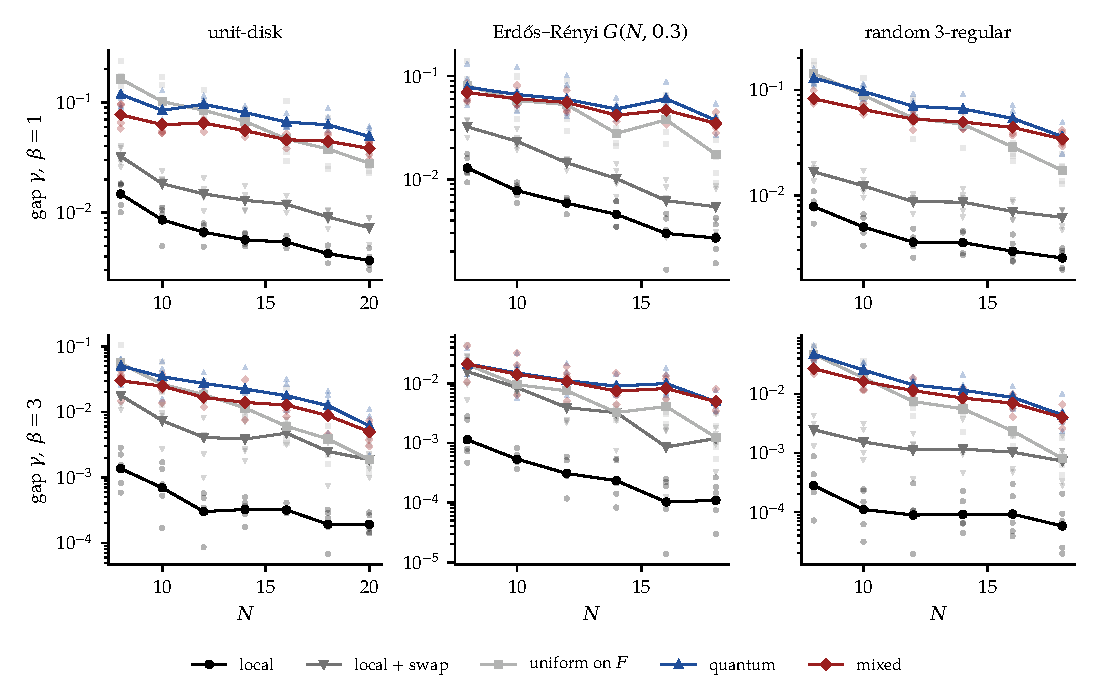
\includegraphics[width=\textwidth]{figures/fig_gaps.pdf}
\caption{Spectral gaps of the five kernels against $N$ for three graph families and two inverse
temperatures. Points are individual instances and lines are geometric means over five seeds.}
\label{fig:gaps}
\end{figure}

\subsection{Spectral gaps}
Figure~\ref{fig:gaps} shows the gaps. Quantum proposals enlarge the gap over local moves in every
instance, by factors between 3.4 and 1116; the geometric means are 25.6 on unit-disk, 20.3 on
Erd\H{o}s--R\'enyi and 48.6 on 3-regular graphs. The relevant question for advantage is scaling, so
we fit $\log\gamma=-\kappa N+c$ and report the ratio $a=\kappa_{\mathrm C}/\kappa_{\mathrm Q}$ against
the best classical kernel. This ratio is the exponent in the relation (classical steps)
$\approx$ (quantum steps)$^a$~\cite{layden2023quantum}.

\begin{table}[t]
\centering\small
\begin{tabular}{@{}lclll@{}}
\toprule
Family & $\beta$ & $\kappa_{\mathrm Q}$ & best classical $\kappa_{\mathrm C}$ & $a=\kappa_{\mathrm C}/\kappa_{\mathrm Q}$\\
\midrule
Unit-disk & 1 & $0.065\pm0.009$ & $0.103\pm0.010$ (local) & $1.60\pm0.28$\\
Unit-disk & 3 & $0.157\pm0.020$ & $0.150\pm0.026$ (local) & $0.95\pm0.21$\\
Erd\H{o}s--R\'enyi & 1 & $0.060\pm0.017$ & $0.137\pm0.023$ (uniform) & $2.28\pm0.76$\\
Erd\H{o}s--R\'enyi & 3 & $0.125\pm0.024$ & $0.242\pm0.042$ (local) & $1.94\pm0.50$\\
3-regular & 1 & $0.118\pm0.011$ & $0.095\pm0.011$ (local+swap) & $0.81\pm0.12$\\
3-regular & 3 & $0.218\pm0.020$ & $0.104\pm0.035$ (local+swap) & $0.48\pm0.17$\\
\bottomrule
\end{tabular}
\caption{Fitted gap-scaling rates with standard errors. Values of $a$ above one favour the quantum
kernel.}
\label{tab:exponents}
\end{table}

Table~\ref{tab:exponents} shows that the scaling behaviour depends on the family. On
Erd\H{o}s--R\'enyi graphs the quantum kernel improves the scaling rate by a factor of about two. On
unit-disk graphs it improves only at high temperature. On random 3-regular graphs the
swap-augmented classical chain scales better than the quantum kernel.

\begin{figure}[t]
\centering
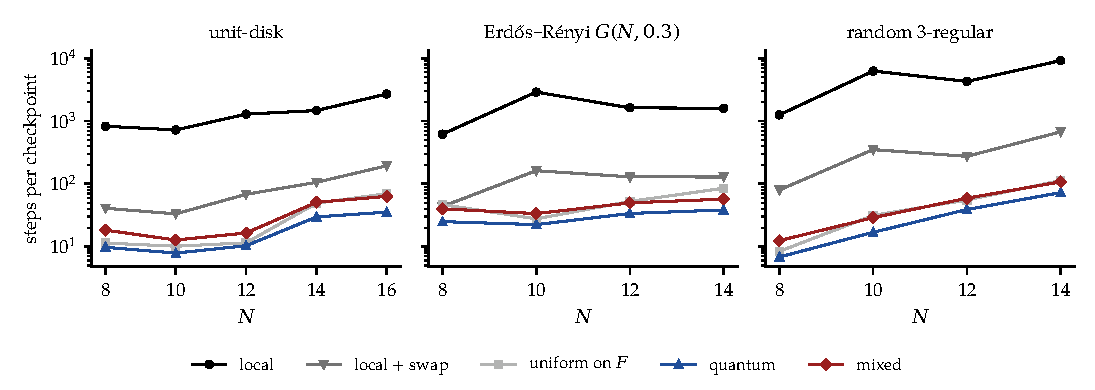
\includegraphics[width=\textwidth]{figures/fig_tracking.pdf}
\caption{Exact warm-start tracking cost: the number of chain steps needed to move from $\pi_t$ to
within $\chi^2\le0.01$ of $\pi_{t+30}$ along multiplicative-weights trajectories ($T=300$,
$\beta=3$). Values are geometric means over three seeds and nine checkpoints.}
\label{fig:tracking}
\end{figure}

\subsection{Tracking along fairness trajectories}
Theorem~\ref{thm:warm} identifies the tracking cost as the operational quantity. For each instance
we generated a multiplicative-weights trajectory with exact Gibbs sampling. For checkpoints thirty
rounds apart, we computed exactly the least number of steps $k$ with
$\chi^2(\pi_tP_{t+30}^k\|\pi_{t+30})\le0.01$. Figure~\ref{fig:tracking} shows the results. The
quantum kernel required the fewest steps in 82\% of the 39 instances. In geometric mean it needed
21.4 steps against 32.3 for uniform proposals, 120.6 for local+swap and 1910 for local moves. Per
instance, the best classical kernel required 1.44 times as many steps as the quantum kernel in
geometric mean. The growth of the tracking cost with $N$ is similar for the quantum and uniform
kernels over the range tested.

\subsection{Repeated max-min allocation}
On the unit-disk instance with $N=12$ and seed 1 ($|F|=131$, three agents), the ex-ante optimum is
$v^*=1.460$ and the best single allocation achieves 1.227. With $\beta=3$, $T=1500$, $k=8$,
$k_0=200$ and five repetitions, Theorem~\ref{thm:dyn} guarantees at least $v^*-0.620$.

\begin{center}\small
\begin{tabular}{@{}llll@{}}
\toprule
Chain & Fairness value & Gini of averages & Dual upper bound\\
\midrule
classical ($q=0$) & $1.179\pm0.139$ & 0.0127 & 1.467\\
quantum-mixed ($q=0.5$) & $1.327\pm0.007$ & 0.0104 & 1.470\\
\bottomrule
\end{tabular}
\end{center}

At equal step budget, the quantum-mixed chain exceeds the best deterministic allocation in every
repetition and reduces the run-to-run standard deviation by a factor of about nineteen. The
classical chain falls below the deterministic optimum in three of five runs.

% =====================================================================
\section{Discussion}

The theory fixes where a quantum device can contribute. Fairness adds no hardness ex ante, and no
representation cost once lotteries are admitted (Theorems~\ref{thm:sep} and~\ref{thm:neutral}). Any
speedup must therefore come from sampling the weighted feasible set, and the warm-start theorem
makes the spectral gap the governing quantity.

The experiments show that constraint-native quantum proposals improve this quantity by large
constant factors in all families and reduce tracking cost in most instances. They improve the
scaling rate on dense random graphs but not on sparse regular ones. For a reversible kernel, the
spectral gap is at most twice the conductance of any set~\cite{levin2017markov,sinclair1989approximate}.
A quantum proposal therefore helps only by moving probability across the bottlenecks of $\pi$, and
the family dependence observed here is consistent with the absence of a generic
mechanism~\cite{orfi2024bounding,orfi2024barriers} and with the finding that part of the
quantum proposal's benefit can be reproduced by quantum-inspired classical
moves~\cite{christmann2025quantum}.

The Erd\H{o}s--R\'enyi ratios of $1.9\pm0.5$ and $2.3\pm0.8$ are consistent with a quadratic-order
improvement. They do not exceed the threshold that error-corrected advantage is estimated to
require~\cite{babbush2021focus}, and they are measured at small sizes.

\paragraph{Limitations.}
\begin{itemize}[leftmargin=*]
\item Instance sizes are limited to $N\le20$ by exact diagonalisation.
\item Parallel tempering~\cite{hukushima1996exchange} and cluster
algorithms~\cite{swendsen1987nonuniversal} were not included, because their gaps are not
computable exactly on the extended state space.
\item Comparisons count chain steps rather than wall-clock cost, and a quantum step costs more than a
classical flip.
\item The uniform baseline is idealised.
\item Hardware noise was not modelled. The proposal is exactly symmetric only for the ideal circuit,
and noise-induced asymmetry would bias the stationary distribution unless mitigated.
\end{itemize}
Extending the study to $N\ge30$ by matrix-free Lanczos methods~\cite{lanczos1950iteration},
adding parallel tempering by autocorrelation measurements, testing non-stoquastic
drivers~\cite{choi2026exponential}, and costing proposals in physical time on Rydberg
hardware~\cite{ebadi2022quantum} would decide whether the Erd\H{o}s--R\'enyi scaling persists.

% =====================================================================
\section{Conclusion}

Fair allocation of indivisible resources admits an exact reformulation in which fairness is a rule
for updating priority weights and computation reduces to Gibbs sampling over the feasible set. This
removes the representability obstruction that has shaped quantum treatments of equity. It also
shows that fairness itself neither creates nor destroys quantum advantage. For fair scheduling under
interference, a blockade-preserving quantum proposal gives an exactly correct sampler with
gate-level resources stated in closed form. It yields large constant-factor improvements, lower
tracking cost in most instances, and an improvement in gap scaling on dense random graphs, which is
instance-dependent rather than general.

\section*{Declarations}
\noindent\emph{Data availability.} All data are generated by the released code from fixed seeds. The
results files are included in the code archive.\\[3pt]
\emph{Code availability.} The complete implementation (fairq, version 1.0.0) with a one-command
reproduction script is provided as supplementary material under the MIT licence.\\[3pt]
\emph{Acknowledgements.} We thank Dr.~Mrittunjoy Guha Majumdar, School of Artificial Intelligence,
Amrita Vishwa Vidyapeetham, Faridabad, for supervising this work.\\[3pt]
\emph{Funding.} No funding was received for this work.\\[3pt]
\emph{Competing interests.} The authors declare no competing interests.\\[3pt]
\emph{Author contributions.} All authors contributed to the theory, the software, the experiments and
the manuscript, and approved the final version.\\[3pt]
\emph{Use of AI tools.} An AI assistant (Claude, Anthropic) was used to support literature search,
drafting and code development. All results were generated by the released code, and the authors
reviewed the content and take full responsibility for it.

% =====================================================================
\section*{Appendix A. The allowed weights of each criterion}

Each entry of Table~\ref{tab:criteria} follows from the conjugate \eqref{eq:conj}.

\noindent\emph{Max-min.} For a probability vector $\theta$, $\theta\cdot y\ge\min_iy_i$, with equality
when all $y_i$ are equal, so $W^*(\theta)=0$. For any other $\theta$ the infimum in \eqref{eq:conj} is
$-\infty$: a negative $\theta_j$ lets $y_j$ grow without bound, and weights that do not sum to one let
a constant vector $y$ run off to $\pm\infty$.

\noindent\emph{Ordered weighted averages and Gini--Sen welfare.} For decreasing $\omega$, the
rearrangement inequality~\cite{hardy1952inequalities} gives $\sum_k\omega_ky_{(k)}$ as the minimum of
$\sum_i\omega_{\sigma(i)}y_i$ over all permutations $\sigma$, so the allowed weights are the
permutations of $\omega$ and their mixtures. Gini--Sen welfare is the case
$\omega_k=(2(n-k)+1)/n^2$, since $\mathrm{mean}\times(1-\text{Gini})=n^{-2}\sum_{i,j}\min(y_i,y_j)$ and
$y_{(k)}$ is the smaller element of exactly $2(n-k)+1$ ordered pairs.

\noindent\emph{Nash.} $\min_{y>0}(\theta y-\log y)=1+\log\theta$, attained at $y=1/\theta$.

\noindent\emph{$\alpha$-fairness.} The minimum is attained at $\theta_i=y_i^{-\alpha}$ and gives
$W^*(\theta)=\frac{\alpha}{\alpha-1}\sum_i\theta_i^{(\alpha-1)/\alpha}$.

\noindent\emph{Linear requirements.} A requirement that is linear in the lottery, such as a need
floor or ex-ante envy-freeness, adds one non-negative multiplier to the weights by Lagrangian
duality~\cite{boyd2004convex}.

\noindent\emph{Which criteria respect Pareto improvements.} A concave $W$ never decreases when some
agent gains if and only if all its allowed weights are non-negative~\cite{rockafellar1970convex}. Mean
minus variance fails this test: its weights $\theta_i=\frac1n-\frac{2\lambda}n(y_i-\mathrm{mean}(y))$
are negative for agents who are well enough off.

\section*{Appendix B. Benchmark instance}

The benchmark is \texttt{make\_instance(20, 3, 0, kind="udg")}. Its edges are
\begin{quote}\footnotesize\ttfamily\raggedright
(0,5) (0,6) (0,7) (0,8) (0,12) (0,15) (0,17) (0,19) (1,10) (2,3) (2,4) (2,11) (2,13) (2,14)
(2,18) (3,4) (3,8) (3,11) (3,12) (3,14) (3,15) (3,18) (4,11) (4,14) (4,18) (5,6) (5,7) (6,7)
(6,19) (7,12) (7,15) (7,17) (7,19) (8,11) (8,12) (8,14) (8,15) (8,19) (9,12) (9,16) (9,17)
(11,12) (11,14) (11,15) (11,18) (12,14) (12,15) (12,17) (12,19) (14,15) (14,18) (15,17) (15,19)
\end{quote}
and its colour classes are $C_1=\{1,2,6,12,16\}$, $C_2=\{4,5,9,10,13,15\}$, $C_3=\{0,3\}$,
$C_4=\{7,11\}$, $C_5=\{14,17,19\}$ and $C_6=\{8,18\}$. The first driver gate of a step, for vertex 1
with $N(1)=\{10\}$, reads in OpenQASM~2.0~\cite{cross2017open}
\begin{quote}\footnotesize\ttfamily\raggedright
x q[10]; h q[1]; cx q[10],q[1]; rz(-0.1) q[1]; cx q[10],q[1]; rz(0.1) q[1]; h q[1]; x q[10];
\end{quote}
The full step is written by \texttt{circuit\_spec.py} to \texttt{results/proposal\_step.qasm}, and the
rates and owners to \texttt{results/circuit\_spec.json}.

\bibliographystyle{abbrvnat}
\bibliography{refs}

\end{document}
